\documentclass{rapport}
\usepackage[utf8]{inputenc}

\usepackage{pifont} % Pour les symboles appelés par la macro \ding
\usepackage{url} % Comme son nom l'indique, pour les url...

\usetikzlibrary{positioning} % Bibliothèque tikz pour positionner des nœuds relativement à d'autres

\usepackage[colorlinks, citecolor=red!60!green, linkcolor=blue!60!green, urlcolor=magenta]{hyperref} % Pour que les liens soient cliquables. Les options permettent de mettre les liens en couleur.

\usepackage{algorithm}
\usepackage[backend=biber]{biblatex}
\usepackage{arevmath}     % For math symbols
\usepackage[noend]{algpseudocode}
\addbibresource{biblio.bib}



\pagestyle{fancy}
\renewcommand{\sectionmark}[1]{\markboth{\thesection.\ #1}{}}
\fancyfoot{}

\fancyhead[L]{\textsl{\leftmark}}
\fancyhead[R, LO]{\textbf{\thepage}}
\fancyhead[RO]{\textsl{\rightmark}}

\def\Latex{\LaTeX\xspace}
\def\etc{\textit{etc.}}


\title{Projet de Neural Networks and Learning}
\author{Antoine Vidal-Mazuy, Jean Philippe Carlens}
\supervisor{Enrico Formenti}
\date{First semester, year 2021-2022}

\formation{Computer Sciences Master} % Nom de la formation

\begin{document}

\maketitle
\tableofcontents


  %%%%%%%%%%%%%%%%%%%%%%%%%
  % Introduction          %
  %%%%%%%%%%%%%%%%%%%%%%%%%
\clearpage
\part{Introdution}

    Les sources du projet sont disponible sur Github sur \href{https://github.com/Brotherta/Facial-Mask-Recognition}{Facial-Mask-Recognition}.
    
    \section{Présentation du sujet}
    
        Dans le cadre de la matière \textbf{Neural Networks and Learning}, nous avons effectué un projet réparti en deux parties indépendantes. 

        Tout d'abord, nous devions développer un logiciel d'annotation d'images. Ce logiciel devait permettre de charger des images et de les annoter avec certaines catégories dans une optique d'utiliser celles-ci pour de la reconnaissance d'images.

        La deuxième partie de ce projet, s'introduit dans une suite logique du développement du logiciel. Nous avons dû utiliser notre logiciel d'annotation, afin de produire un jeu de données, comprenant des images de personnes avec ou sans masque. Le but final étant de reconnaître et de localiser sur une image, les personnes avec ou sans masque.
    
    \section{Présentation des membres du projet}
    
        Les membres ayant participé à la réalisation de ce projet sont:
        
        \begin{itemize}
            \item Antoine Vidal-Mazuy
            \item Jean-Philippe Carlens
        \end{itemize}
    
    \section{Partage des tâches et gestion du projet}
    
        Nous avons travaillé de manière séparée sur le projet, hormis quelques séances de mise en commun ou de définitions des tâches. Pour cela nous avons utilisé \textit{git} ainsi que \textit{Github} \href{https://github.com/Brotherta/Facial-Mask-Recognition}{Facial-Mask-Recognition}.

        Afin d'éviter de se marcher dessus, nous avons utilisé un KanBan dans \textit{Github}, cela nous a permis de créer des tâches et de s'assigner sur les différentes caractéristiques du projet. La séparation des tâches était ainsi plus naturelle et intuitive pour la première partie du logiciel, ainsi chacun s'occupait d'une partie. Pour la deuxième partie, nous avons dû rechercher chacun de notre côté, et mettre en commun par la suite. Nous nous sommes également réparti les différentes expérimentations d'entraînement du modèle.
    \clearpage
    
\part{Logiciel d'annotation}

    \section{Introduction du logiciel}
        
        \subsection{Instruction d'utilisations}
        
        Vous pouvez voir les instructions d'utilisations du logiciel sur ce \href{https://github.com/Brotherta/Facial-Mask-Recognition/blob/main/README.md}{lien}.
        
        \subsection{Cahier des charges}
        
            Le logiciel devait répondre à certaines caractéristiques que nous allons citer ici:

            \begin{itemize}

                \item \textit{Charger des image}. Le logiciel doit permettre de charger des images au format \textit{jpeg} et \textit{png}.

                \item \textit{Charger des catégories}. Le logiciel doit permettre de charger depuis un fichier \textit{json} ou \textit{csv}, différentes catégories.

                \item \textit{Créer des catégories}. Créer des catégories semble essentiel, elles sont donc sauvegardées dans un fichier \textit{json} qui pourront être réutilisés dans un autre projet.

                \item \textit{Annoter des images}. Les images chargées, doivent pouvoir être visualisées, et annotées à l'aide de cadres dessinés par l'utilisateur. Les annotations doivent être sauvegardées dans un fichier \textit{json} afin d'être réutilisées plus tard.

                \item \textit{Unifier} des types des images. Afin de garder une cohérence dans le jeu de données créé, il est important que les images importées soient toutes sauvegardées dans un type équivalent.

                \item \textit{Cohérence} des annotations. Les cadres doivent respecter quelques caractéristiques comme des tailles minimales, ou encore ne pas trop se chevaucher entre eux.
                
            \end{itemize}
                    
        \subsection{Technologies utilisées}
        
            Nous nous sommes servis de \textbf{\textit{Python}} pour développer le logiciel. Pour aider au développement, nous avons également utilisé plusieurs autres librairies python\space:
            
            \begin{itemize}
                \item Pour la gestion des images, nous avons utilisé la librairie \href{https://pillow.readthedocs.io/en/stable/}{\textit{Pillow}} ainsi que \href{https://pillow.readthedocs.io/en/stable/}{Open-CV}. Ces librairies nous ont permis de faciliter l'ouverture, la modification ainsi que la sauvegarde des images. Le sujet nous recommandait l'utilisation de la librairie \href{https://pillow.readthedocs.io/en/stable/}{\textit{Shapely}}, pour faciliter la manipulation des intersections de formes géométriques. Cependant nous l'avions oublié, et avons développé notre propre fonction. Nous sommes très satisfaits du résultat, et avons ainsi décidé de garder cette dernière et de nous passer de \textit{Shapely}.

                \item Au niveau de l'interface graphique, nous avons opté pour \href{https://www.qt.io/}{\textit{Qt}}, et de son portage python \href{https://pypi.org/project/PyQt5/}{\textit{PyQt5}}, au détriment de \textit{tkinter}, pour lequel nous avions eu quelques expériences décevantes par le passé. \textit{Qt} est complet, rapide, et très bien documenté. Nous voulions donc profiter de ce projet pour polir nos compétences dans l'utilisation de ce framework.

                \item Pour la lecture et écriture des fichiers \textit{CSV}, nous avons utilisé \href{https://pandas.pydata.org/}{Pandas} que nous avons pu découvrir durant ce cours et qui facilite grandement le traitement des données.
            \end{itemize}   
        
        \subsection{Modèles Model-View-Controller}
        
            \subsubsection{Introduction}
            Nous avons durant ce projet attaché beaucoup d'importance à la propreté ainsi qu'à la structuration de notre code. Nous avons donc décidé d'apprendre et d'implémenter un patron de conception très populaire dans le monde des interfaces graphiques : le pattern \href{https://en.wikipedia.org/wiki/Model\%E2\%80\%93view\%E2\%80\%93controller}{\textit{MVC}}, pour \textbf{Model-View-Controller}.
        
            \subsubsection{Le fonctionnement}
            Le principe du pattern \textit{MVC} est de diviser le code en 3 modules différents, qui auront chacun une responsabilité qui leur sera propre : 
            
            \begin{itemize}
                \item Le module \textbf{\textit{Model}}, qui s'occupe du stockage, de la lecture et de l'écriture des données du programme. C'est donc ici qu'il y aura les définitions de nos images. de nos labels, de nos projets et ainsi de suite. Il est indépendant des deux autres modules.

                \item Le module \textbf{\textit{View}}, qui va contenir toute la partie \textbf{visible} de notre interface graphique. Il va afficher nos fenêtres, dialogues, menus et donc de communiquer avec l'utilisateur. La vue ne fait que recevoir des informations et les afficher, et signaler les interactions avec l'utilisateur. Il dépend donc uniquement du module \textit{Model}.

                \item Le module \textbf{\textit{Controller}}, qui lui va faire la liaison entre les deux modules précédents. Comme un cerveau, il va recevoir par le biais du module \textit{View} les actions de l'utilisateur, puis modifier les données dans le module \textit{Model} et mettre à jour le module \textit{View} en conséquence.  
            \end{itemize}
            
            Cette répartition nous permet d'éviter un effet \textit{"spaghetti"} dans notre code et va donc grandement faciliter la maintenance, l'ajout de fonctionnalité ainsi que de réduire drastiquement la probabilité d'obtenir un logiciel bugué.
            
            \subsubsection{Qt et le MVC}
            \textit{Qt} facilite grandement l'intégration du pattern \textit{MVC}. C'est ainsi que nous avons pu utiliser un système de notifications, très utile, qui va notamment permettre à notre module \textit{View} d'envoyer des signaux au module \textit{Controller}, en l'occurrence pour signaler les actions de l'utilisateur, sans pour autant en dépendre et donc importer tout le module. Cela va nous permettre de respecter les règles de dépendances du pattern \textit{MVC} et de garder ainsi un code aussi épuré que possible.
            
    \section{Réalisation}
    
        \subsection{Projet et environnement}
        Le logiciel se repose sur un système de gestion de projet. Il demandera ainsi à l'utilisateur s'il veut créer ou charger un projet déjà existant, et affichera une liste de projets récents, tout en s'efforçant par la même occasion d'afficher uniquement ceux qui sont valides. Signalant ainsi à l'utilisateur la détection et donc suppression de projets corrompus.

        Une fois un projet ouvert, un environnement sera proposé à l'utilisateur, lui affichant la liste des images et des catégories du projet. Il aura ainsi à sa disposition divers outils pour manipuler le tout.

        Nous avons également implémenté un système de thème, laissant à l'utilisateur le choix entre un affichage sombre ou lumineux.
        
            \subsubsection{Constitution d'un projet}
            Un projet est constitué de 4 éléments : 
            \begin{itemize}
                \item \textbf{\textit{project.ini}}, le fichier mère qui va contenir les chemins vers les autres fichiers/dossiers d'informations du projet, ainsi que son nom.
                
                \item \textbf{\textit{images/}}, le dossier qui va contenir toutes les images qui seront chargées et ajoutées au projet.
                
                \item \textbf{\textit{box.json}}, le fichier qui va contenir toutes les annotations de notre projet, représentées par une liste d'objets, contenant le lien vers leur image et leur liste de cadres associés.
                
                \item \textbf{\textit{labels.json}}, le fichier qui va contenir la liste des catégories pouvant être annotées dans le projet courant.
            \end{itemize}
            
            Dans notre code, la classe du module \textit{Model}, \textbf{\textit{Project}}, s'occupe de contenir, charger et sauvegarder un projet.
            La classe \textbf{\textit{ProjectController}}, du module \textit{Controller}, s'occupe elle de gérer le projet de faire le lien entre les données entre l'interface graphique de création et chargement de projet, avec le module View et sa classe \textit{ProjectWindow}.
    
    
            \subsubsection{Processus de création d'un projet}
            Lorsque l'utilisateur clique sur le bouton \textit{"New Project"}, un dialogue apparaît, demandant à l'utilisateur de spécifier nom et emplacement de ses sauvegardes. Il devra spécifier un dossier vide, à l'aide d'un dialogue qui ouvrira l'explorateur de fichier. Une fois créé, le projet sera ajouté à la liste des projets récents et pourra donc être chargé par l'utilisateur.
    
            C'est ici non pas le \textit{ProjectController} mais le \textit{MainController} qui va s'occuper de récupérer l'action d'ouverture d'un projet, et ainsi de lancer l'ouverture de ce dernier. Il fermera donc la \textit{ProjectWindow} et ouvrira la \textit{MainWindow}, que nous allons étudier par la suite.
    
    
            \subsubsection{Oubli de sauvegarde}
            Lorsqu'un projet sera ouvert, le programme s'efforcera de détecter automatiquement si des modifications ont été opérées par l'utilisateur. L'utilisateur devra sauvegarder manuellement son travail, cependant s'il serait amené à fermer le programme sans sauvegarder, ce dernier captera l'évènement et notifiera cet oubli à l'utilisateur. Il aura donc le choix entre sauvegarder ou non. Nous n'avons pas implémenté de sauvegarde automatique par peur d'impact néfaste sur la performance et la fluidité du programme. Nous avons donc ajouté cette sécurité pour garantir une utilisation satisfaisante du logiciel. Nous reviendrons sur le fonctionnement de la sauvegarde par la suite.
            
            \subsubsection{Environnement de travail}
            L'environnement de travail principal repose sur la \textit{MainWindow}. Cette dernière se divisera en trois composantes principales :
            
            \begin{itemize}
                \item La barre de menus, sur la partie supérieure de la fenêtre. En premier lieu nous avons le menu \textit{File} qui va contenir les boutons d'importations d'image et de catégorie, ainsi qu'un bouton de sauvegarde du projet.
    
                Viens ensuite le menu \textit{"New"} qui va simplement contenir le bouton de création de catégories, pour les annotations. En troisième nous avons un bouton \textit{"Help"} qui pourra rediriger l'utilisateur vers le \href{https://github.com/Brotherta/Facial-Mask-Recognition/blob/main/README.md}{README.md} de notre dépôt \textit{GitHub}. Et finalement, le menu \textit{"Settings"} qui pourra donner à l'utilisateur le choix du thème de l'interface graphique. Le code de la barre de menus se trouve dans notre classe \textit{MenuBar}, qui hérite de la \textit{QMenuBar} de Qt.
    
                \item Sur la partie gauche de la fenêtre, nous avons une liste verticale des catégories pouvant être annotées dans le projet. Nous pouvons, à l'aide d'un clic droit, créer, supprimer, et même renommer une catégorie existante. Cette dernière action verra toutes les annotations existantes mises à jour. Le code se trouve dans notre classe \textit{ImageListWidget}.
    
                \item Dernièrement, sur la droite de la fenêtre et prenant la majorité de la place, la liste des miniatures des images importées au projet. Il suffira ainsi de double-cliquer sur une image pour en ouvrir l'éditeur d'annotation. L'utilisateur pourra sélectionner une ou plusieurs images simultanément et les supprimer à l'aide du bouton associé ou lors d'un clic droit. Le code ici se trouve dans la classe \textit{LabelsWidget}.
            \end{itemize}
        
        \subsection{Catégories}
        Le programme veillera à éviter que l'utilisateur ne créer de catégorie doublon, ainsi que du renommage intelligent des catégories et de leurs annotations associées, comme évoqué précédemment. Lors de la sauvegarde, elles seront écrites dans le fichier \textit{labels.json}. Ce dernier qui sera, bien entendu, chargé à chaque ouverture de projet. Les catégories seront représentées par la classe \textit{Label} du module \textit{Model}.
        
        \subsection{Images}
        Les images importées au projet seront automatiquement copiées dans le dossier \textit{images/}. Ensuite, nous chargons ces images dans notre classe \textit{ImageFMR} du module \textit{Model}.


        Cette classe va encapsuler le chemin de l'image, et renvoyer si nécessaire à la demande de l'utilisateur l'image chargée dans un \textit{QPixmap} de \textit{Qt} (L'objet d'une image dans le framework \textit{Qt}) ou une icône \textit{QIcon}, une version miniaturisée de l'image. Elle met également à la disposition de l'utilisateur une méthode de redimensionnement, qui vérifie si l'image dépasse notre résolution limite (1200x675), et la réduit en conséquence.


        Elle va également encapsuler la liste des annotations associées à l'image. Cela se caractérise par une liste d'instance de la classe \textit{Box}, que nous allons évoquer par la suite. On pourra donc via une méthode, ajouter de nouvelles zones d'annotation à l'image.
        
        \subsection{Annotation des Images}
        C'est dans l'éditeur d'image que nous pourrons annoter nos images. Il sera très simplement constitué d'un dialogue affichant l'image, et deux boutons en dessous : valider et annuler. L'utilisateur pourra ainsi dessiner des cadres en maintenant clic gauche. L'ouverture d'une image existant déjà au préalable affichera bien sûr les cadres éventuellement déjà créés et sauvegardés par le passé. Ils sont représentés dans notre code par la classe \textit{Box} évoquée précédemment, qui encapsule les quatre valeurs représentant un rectangle (coordonnées du point supérieur gauche, longueur et largeur), et l'objet \textit{Label} représentant l'annotation associée au cadre.

            \subsubsection{Cadres}
            Les cadres représentent nos annotations. Ils ont 2 couleurs possibles : blanc pour non annoté et vert foncé pour annoté. Lors d'un double-clic sur un cadre, une boîte de dialogue s'affiche avec 3 widgets.

            Premièrement une liste déroulante des catégories pouvant être associée au cadre. Si une catégorie a déjà été associée, elle sera affichée en première dans la liste, ce qui nous permet de voir quelle est la catégorie déjà associée. Ensuite deux boutons, l'un pour supprimer le cadre, et le deuxième pour confirmer l'association de la catégorie à l'annotation.

            Les annotations peuvent être sauvegardées même sans catégorie associée.

            \subsubsection{Implémentation de la zone de dessin}
            Pour permettre a l'utilisateur de dessiner avec la souris, nous avons créé une classe, \textit{QLabelFMR} qui hérite de la \textit{QGraphicsView} de \textit{Qt}.
            Cette classe va nous permettre de pouvoir dessiner des formes géométriques par-dessus des images déjà existantes. 
            Nous allons ainsi grâce à \textit{Qt} capturer les évènements de la souris et agir en fonction. Voici la procédure :

            \begin{enumerate}
                \item Nous récupérons les évènements de clic gauche, et nous en sauvegardons l'emplacement.

                \item Nous récupérons les évènements de déplacement de la souris. Si la souris se déplace et qu'un emplacement de clic gauche ait été sauvegardé et donc non nul, alors l'utilisateur est en train de déplacer la souris tout en maintenant le clic gauche (lors du relâchement du clic nous nullifions l'emplacement).

                À chaque évènement de déplacement, nous effaçons s'il existe déjà et dessinons le cadre, qui s'étend de l'emplacement du premier clic gauche jusqu'à la coordonnée actuelle du déplacement de la souris.

                \item Nous récupérons les évènements de relâchement de boutons de la souris. Si le bouton relâché est le bouton gauche, et qu'un cadre a été dessiné auparavant, nous vérifions que les dimensions du cadre sont valides. Si le cadre est invalide, nous le supprimons.

            \end{enumerate}

            \subsubsection{Coordonnées et conflits}
            Nous avions évoqué en parlant du relâchement de la souris de la vérification et la validité des coordonnées du cadre. En effet, nous vérifions, comme demandé dans le sujet, qu'il face au minimum 5 pixels de longueur et de largeur, ainsi que de 40 pixels d'aire. Nous vérifions également, à la main et donc sans Shapely comme expliqué dans l'introduction, les collisions avec les autres cadres. En accord avec le sujet, si le nouveau cadre partage 20\% sur de la surface d'un cadre déjà existant, alors il est invalide.

            \subsubsection{Sauvegarde du cadre}
            Si l'utilisateur décide de cliquer sur annuler, alors tout le travail d'édition sera oublié. S'il choisit l'option validée, alors le travail sera enregistré en mémoire vive avec le reste du projet.
            
        \subsection{Sauvegarde et chargement du projet}

            \subsubsection{Introduction}
            Nous avons dans l'écrasante majorité des cas opté pour le format \textit{json} pour enregistrer nos données. Cela nous a facilité la tâche car il existe des solutions très simples pour parser nos objets tels quels au format \textit{json} via la librairie standard de \textit{python}. En l'occurrence, nous avons utilisé \textbf{\textit{"SimpleNamespace"}}.

            \subsubsection{Chargement de la configuration du projet}
            L'exception est le fichier project.ini qui lui est dans un format \href{https://en.wikipedia.org/wiki/YAML}{\textit{YAML}}. C'est un format de fichier très utile pour les fichiers de configuration, et va nous permettre de très simplement associer des valeurs à des clés, comme dans un dictionnaire. Le module \textit{"configparser"} va ainsi permettre de charger les valeurs du fichier automatiquement dans un dictionnaire \textit{python}, mais aussi de sauvegarder dans le sens inverse.

            \subsubsection{Sauvegarde des annotations}
            Nous sauvegardons nos cadres d'annotation et nos catégories dans des fichiers \textit{json}. Pour cela, nous devons avoir un moyen de parser nos données dans ce format. Pour cela, nous avons utilisé \textit{SimpleNamespace} qui va automatiquement rendre notre classe convertible. Ainsi, lorsque nous voulons sauvegarder notre travail, nous faisons deux simples appels à la fonction \textbf{json.dumps()}, le premier nous lui donnons en argument notre liste d'\textit{ImageFMR} (notre classe encapsulant les images et leur liste de cadres associés), et le second la liste de catégories (notre classe Label). Nous sauvegardons les chaînes de caractères retournées dans leurs fichiers respectifs (\textit{box.json} et \textit{labels.json}).

            \subsubsection{Système de vérification d'oubli de sauvegarde}
            Nous avions évoqué auparavant un système de prévention d'oubli de sauvegarde.
            Le fonctionnement est très simple. Lors du chargement des fichiers \textit{"box.jsons"} et \textit{"labels.json"}. Nous concaténons les deux chaînes de caractères représentant leurs contenus respectifs en une seule chaîne.
            Ensuite, lors de la fermeture du programme, nous faisons la même opération mais avec les annotations et catégories en mémoire vive. En comparant les deux concaténations, nous pouvons savoir si l'état du projet actuel diffère de celui au moment du chargement.
            
    \section{Problèmes rencontrés}
    Nous avons bien évidemment rencontré divers problèmes durant ce projet. Nous allons ici les aborder.
    
        \subsection{Portabilité du programme}
        Nous avons eu quelques soucis de portabilité dont l'origine nous est inconnue. Notre programme est est en effet optimal sur Windows. En effet, lors de l'import d'image au projet, nous affichons un dialogue avec une barre de progression dans un thread différent, affichant la progression des imports image par image. Le code marche parfaitement sur Windows, mais crash sur macOS. Nous avons donc dû détecter l'OS de l'utilisateur et lancer ou non la barre de progression en fonction. Il est utile de préciser que le seul mac en notre disposition est un mac tournant sur un processeur ARM. Nous ignorons donc si le problème vient spécifiquement de mac OS ou de l'architecture du processeur.

    
        Nous avons également constaté, durant la partie 2, que le programme pouvait tout simplement ne pas se lancer sur Linux pour une raison que nous ignorons, mais nous manquons de données pour savoir si cela est le cas chez tout le monde, et/ou sur quelles distributions. Cela pouvait également être un problème personnel.

        \subsection{Ergonomie du programme}
        Nous nous sommes rendu compte, en abordant la partie 2 du projet, que nous n'avions pas assez testé notre programme en condition réelle d'utilisation, en se mettant réellement du point de vue de l'utilisateur. C'est donc en utilisant sérieusement le programme sur un nombre très important d'images que nous nous sommes rendu compte que l'ergonomie du programme pouvait être encore bien améliorée. Par exemple, un système d'annotation automatique, où les cadres auront par défaut automatiquement la dernière catégorie employée.

        \subsubsection{Failles passées inaperçues}
        Nous nous sommes également rendus compte d'un bogue qui est passé étrangement entre les mailles du filet.
        En effet, si l'on dessine un ou plusieurs cadres sur plusieurs images, nous ne pouvons pas consulter les anciennes images éditées, sous peine de crash. La faute à notre manque de test sur les toutes dernières versions du logiciel. Ce souci a été très vite résolu, mais malheureusement après le rendu de la première partie.

        \subsection{Quelques pièges de python}
        Nous avons aussi été confrontés à quelques soucis improbables. Mais après renseignement, nous avons trouvé que le \textit{Garbage-Collector} de python pouvait, dans certaines situations précises, détruire des données que nous utilisions encore avec \textit{PyQt}. Nous avons pu régler ce genre de soucis par l'utilisation de variables globales par exemple.

    \clearpage
\part{Classificateur d'images avec masque / non masque}

    \section{Introduction}
    
        \subsection{Instructions d'utilisations}
            
            Le programmes peut se lancer via un terminal, ou encore via le logiciel.
            
            Pour la partie logiciel, il suffit d'aller dans la barre des menus dans la section "\textbf{Model}". \textbf{Rappel}, pour lancer le logiciel, il faut lancer en ligne de commande le script python \textbf{app.py}. Pour l'utlisation du logiciel, nous vous renvoyons vers le tuto \href{https://github.com/Brotherta/Facial-Mask-Recognition/blob/main/README.md}{ici}. Pour la partie d'entraînement des modèles, plusieurs actions sont disponibles :
            
            \begin{itemize}
                \item  \textbf{Create a new model from annotations} : Ce mode permet de lancer le pré-traitement des données, via un  fichier d'annotations json créé par le logiciel. Il suffit de selectionner un fichier \textit{box.json} d'un projet quelconque, et de rentrer un nom pour le modèle ainsi créé. L'entraînement sera ensuite lancé automatiquement. Attention l'évolution de l'entraînement est disponible uniquement à travers le terminal.
                
                \item \textbf{Create a new model from existing images} : Ce mode est similaire au précédent, à la différence qu'il n'y a pas de pré-traitement fait sur les images.
                
                \item \textbf{Load a model} : Ce mode permet de charger en mémoire un modèle. Il est nécessaire, d'effectuer cette action avant de lancer la prédiction.
                
                \item \textbf{Stop the running training} : Ce mode permet en théorie d'arrêter l'entrainement en cours. En réalité cela ferme entièrement le programme, car nous n'avons pas accès à l'intérieur de la méthode \textit{fit} de keras.
                
                \item \textbf{Predict images} : Ce mode permet à l'utilisateur de sélectionner des images à prédire. Attention, il faut avoir chargé en mémoire un modèle au préalable.
                
            \end{itemize}
            
            Pour la partie terminal, vous devez lancer le script avec la commande suivante :
            \textbf{python main\_predictor.py}
             \begin{itemize}
                 \item \textbf{-{}-mode} \textbf{\textit{preprocess}} \textbf{-{}-path} \textit{CHEMIN\_VERS\_FICHIER\_ANNOTATION}.
                 Spécifier le chemin avec \textit{-{}-path} est \textbf{obligatoire} dans ce cas. Cela doit être un fichier d'annotations crée par notre logiciel de la partie 1. Il faut spécifier le fichier \textit{box.json}.
                 
                 \item \textbf{-{}-mode} \textbf{\textit{train}} (\textbf{-{}-path} \textit{CHEMIN\_VERS\_DOSSIER}).
                 Spécifier le dossier avec -\textit{-{}-path} est ici facultatif, par défaut le programme sélectionnera le dossier \textit{resized\_images/}. Si spécifié, le dossier doit contenir deux sous dossier représentant les images avec et sans masques, \textit{mask} et \textit{no\_mask}. Les images trouvées seront redimensionnées.
                 
                 \item \textbf{-{}-mode} \textbf{\textit{predict}} \textbf{\textit{-{}-path}} \textit{CHEMIN\_VERS\_IMAGE} (\textbf{\textit{-{}-model}} \textit{CHEMIN\_VERS\_MODEL}).
                 Spécifier le chemin de l'image est \textbf{obligatoire}. Spécifier le chemin d'un modèle est facultatif, cela permet à l'utilisateur de sélectionner un autre modèle que celui par défaut. Une petite fenêtre va s'ouvrir et afficher l'image donnée ainsi que les cardres de visages masqués détectées.
             \end{itemize}
        
            
        \subsection{Cahier des charges}
            
            Dans cette deuxième partie, nous avions aussi plusieurs tâches à réaliser. En effet, le classificateur devait implémenter plusieurs fonctionnalités dont: 
            
            \begin{itemize}
                \item La création d'un jeu de données. En effet, nous devons constituer un jeu de données comprenant des images de personnes avec ou sans masques. Ce jeu de données doit pouvoir être utilisé par la suite dans notre logiciel d'annotation.
                
                \item La reconnaissance d'une personne portant un masque ou non. En effet le programme doit pouvoir reconnaître sur une image comprenant une personne, si elle porte un masque ou non.
                
                \item La détection des visages sur l'image. Le programme, doit pouvoir localiser les visages, afin de les traiter ensuite pour reconnaître si la personne porte un masque ou non.
                
            \end{itemize}
        \subsection{Technologies utilisées}
        
            Pour cette deuxième, nous avons principalement utilisé la libraire \href{https://keras.io/}{Keras}, qui s'appuie sur Tensorflow\cite{KerasInstall}. Cette librairie nous permet d'utiliser différentes couches pour notre réseau de neurones, mais aussi de le manipuler, afin d'entraîner des modèles. Nous avons pu ensuite utiliser la librairie \href{https://opencv.org/}{\textit{Open CV}}, qui nous permet d'afficher nos images et de rajouter les cadres prédits. Cette libraire est aussi utile, car elle donne accès à un algorithme de \textit{\textit{Selective Search}} que l'on a pu utiliser pour la détection de visage. Enfin nous avons utilisé un \href{https://github.com/anasbadawy/Face-Detection}{modèle pré-entraîné} pour la détection des visages, qui s'appuie sur la fonctionnalité d'\textit{Open CV} évoquée précédemment.
            
        \subsection{Structure du programme}
        
            Notre programme peut se découper en 3 parties. La première partie, s'occupe du pré-traitement des images. La deuxième quant à elle s'occupe de la création du modèle et de l'entraînement. Enfin on termine par la prédiction sur les images.
            
            La première partie va tout d'abord, en fonction du jeu de données, passer par plusieurs étapes. Si le jeu de données sélectionné provient des annotations du logiciel, nous allons tout d'abord lire le fichier \textit{json} de part en part, afin de récupérer et de rogner les images en fonction des cadres.
            
            Une fois les images correctement triées, nous allons pouvoir passer à la création du modèle. Le modèle est ainsi créé en fonction du nombre de sorties possibles. En effet comme nous le détaillerons plus tard, le modèle s'adapte en fonction du nombre de classes possibles.
            
            Enfin, nous pouvons donner les images en entrée de notre modèle pour qu'il s'entraîne à reconnaître les différentes caractéristiques. Une fois l'entraînement terminé, nous pouvons sauvegarder le modèle dans un fichier, afin de pouvoir par la suite prédire des images.
            
            La prédiction passe tout d'abord par un modèle déjà entraîné à reconnaître les visages. Nous récupérons en sorties les visages, et nous donnons à notre modèle le visage en question. Il peut ainsi déterminer si le visage porte un masque ou non.
            
        \subsection{Utilisation du classificateur}
        
            Notre programme est indépendant, du logiciel, et peu être lancé en ligne de commande en lançant le scripts python \textit{main\_predictor.py}. Il y a plusieurs mode de lancement, détaillé dans la documentation du programme. 
            
            \begin{itemize}
                \item  mode \textbf{preprocess}\space: ce mode suivit d'un chemin d'un fichier d'annotations, permet de rogner les images et de les déplacer dans les bons sous-dossier d'entraînement.
                
                \item mode \textbf{train}\space: ce mode permet au modèle sélectionné, de s'entraîner sur le jeu de donnée préalablement pré-traité. Nous pourrons observer dans le terminal, les différentes sorties données par la librairie Keras, et ainsi observer l'avancement de l'entraînement.
                
                \item mode \textbf{predict}\space: ce mode suivit d'un chemin vers une image, permet à l'utilisateur de lancer une prédiction sur une image. On pourra alors observer l'image, avec les cadres identifiés comme masque sur l'image.
                
            \end{itemize}
           
           Bien que, le programme soit fonctionnel dans cet état, nous avons décidé de l'intégrer dans le logiciel d'annotation. Ainsi, il est possible de lancer toutes ces fonctions depuis le logiciel. Nous pouvons retrouver toutes ces fonctionnalités à travers le menu \textit{Model} intégré dans la barre des menus du logiciel. Le déroulement de l'entraînement s'affichera dans le terminal ayant lancer le programme. Attention, les modes d'entraînement sont disponibles dans le logiciel, cependant, nous recommandons de lancer l'entraînement dans un terminal, plutôt qu'à travers le logiciel. En effet, le mode entraînement nécessite beaucoup de ressources CPU. Cela arrive lors de la manipulation du logiciel, si un mode entraînement est lancé, qu'il plante ou qu'il soit très lent. Cependant, la prédiction est intuitive dans le logiciel.
            
        
    \section{Réalisation}
    
        \subsection{Données}
        Il est nécessaire en vue de notre entraînement de pouvoir fournir au programme des données propres et exploitables. C'est pourquoi nous avons dû au préalable effectuer tout un travail de pré-traitement de celles-ci. Nous avons utilisé environ 600 images (300 avec masques et 300 sans). Ensuite, nous avons utilisé notre logiciel d'annotation, afin de définir les cadres ainsi que les labels associés pour chaque image. Nous avons fait très attention à ne garder que les éléments essentiels. En effet nous gardions uniquement le visage, en évitant d'inclure trop de décors, ou encore d'éviter de mettre les cheveux, les casquettes etc...
        
            
            \subsubsection{Choix de format d'image et de résolution}
            Avant toute chose nous devions choisir les caractéristiques que partageront toutes nos données, par souci d'unicité. Le sujet nous recommandait n'importe quelle résolution carrée entre \textbf{120x120} et \textbf{180x180}.
            Nous avons testé ces deux bornes, et n'avons pas trouvé de différences flagrantes si ce n'est le temps d'entraînement. Nous avons donc opté pour la première. Quant au format de l'image, nous avons compris que le format \textit{JPEG} ne poserait aucun souci peu importe les librairies. C'était peut-être également le cas du format \textit{PNG}, mais n'ayant rencontré aucun souci avec \textit{JPEG}, nous avons finalement gardé ce format.
            
            \subsubsection{Récupérer les images d'un projet d'annotation}
            Premièrement nous avons commencé par programmer une petite fonction \textit{python} permettant, à partir d'un fichier \textit{JSON} sauvegardant les annotations d'un projet, de récupérer les informations de chaque image. Nous avons ainsi pour chaque image, le chemin du fichier correspondant ainsi que tous ses cadres d'annotations. Notre script va donc charger l'image, couper les cadres et les enregistrer individuellement dans des fichiers séparés, dans le répertoire de travail. La catégorie annotée du cadre ainsi que la résolution de l'image sera spécifiée dans le nom du fichier, comme indiqué dans le sujet. Toutes les images sont importées et converties s'il le faut au format \textit{JPEG}, dans un dossier nommé \textit{\textbf{"box\_images"}}.
            
            \subsubsection{Redimensionnement des images}
            En second lieu, Nous redimensionnons les images importées dans le cas où elles ne dépasseraient pas notre taille limite, ici \textbf{120x120}. Après cette vérification, les images sont finalement sauvegardées dans le dossier \textbf{\textit{"resized\_images"}}.
            
            \subsubsection{Sets de données train et test}
            Il est important de ne pas entraîner et tester le programme sur les mêmes données. Ainsi nos jeux de données contiennent de base deux dossiers, \textbf{\textit{train}} et \textbf{\textit{test}}. Le premier servira à fournir notre programme en ressources pour son entraînement tandis que le second sera la cible des prédictions du programme, une fois prêt.
            
        \subsection{Détection d'objets}
            Notre programme s'est entraîné sur des petits cadres comportant un seul visage bien coupé. Cependant, nous voulons qu'il soit capable de reconnaître et d'indiquer plusieurs visages masqués sur une image. Nous devons pour cela trouver un moyen de détecter et couper chaque visage, que nous fournirons chacun individuellement à notre fonction de prédiction. La recherche d'une telle méthode nous a pris un temps assez conséquent.
            
            \subsubsection{Open CV Selective Search}
            Nous avons en premier lieu décidé d'opter pour la solution de détection d'objet d'OpenCV. En effet, une fonction nous permettait de nous proposer un nombre conséquent de zone dans l'image présentée comme possibles objets. Il ne nous rester plus qu'à récupérer ses zones et les soumettre au prédicteur : si le résultat est favorable, nous affichons le rectangle. Cependant, les résultats étaient très mitigés et instables. Nous avions beaucoup de zones superposées, et les visages n'étaient clairement pas tout le temps proposés. Nous fournissions ainsi des données souvent incohérentes à notre prédicteur vis-à-vis de son entraînement. De plus, l'analyse de plusieurs milliers de potentielles zones était assez gourmande, et le temps d'analyse des images se comptait en secondes. Nous avons donc décidé de chercher une autre solution.
            
            \subsubsection{Détection de visages par machine learning}
            Voyant le temps défiler, nous essayions le plus possible de ne pas réinventer la roue. Ainsi, nous avons cherché des dépôts \textit{GitHub} de détection de visage que nous pourrions réutiliser. Nous sommes ainsi tombés sur un logiciel\cite{gitFace} qui s'est entraîné, d'une manière similaire à notre projet, à détecter les visages humains, en se basant sur la même technologie que nous utilisions précédemment. Nous avons donc téléchargé les quelques lignes de code et le modèle stockant l'entraînement.

            Ainsi, il nous suffit désormais d'envoyer l'image à une fonction et celle-ci nous retournera les boudings boxs des visages humains potentiels de l'image. Les résultats sont très corrects, et la fonction propose très précisément dans diverses positions les visages humains, même avec divers obstacles pouvant entraver la détection, comme des chapeaux, masques, lunettes et autres. Nous avons donc décidé de garder cette option.
            
            \subsubsection{Lien entre la détection et la prédiction}
            Pour faire la transition, nous parcourons chaque rectangle proposé par la fonction de détection. Cette dernière nous fournit également son pourcentage de confiance en son résultat. Ainsi, s'il y a au moins \textbf{50\% de confiance}, nous utilisons \textit{Open CV} pour copier en mémoire vive la coupe du rectangle proposé. \textit{Keras} utilise des images \textit{PIL} tandis que nous avons actuellement une image \textit{Open CV}. Toutes deux sont traitées de manière différente, c'est pourquoi nous devons manipuler notre petite image pour la rendre compréhensible par \textit{PIL}. C'est pourquoi nous la convertissons du format \textit{\textbf{BGR}} vers le format \textit{\textbf{RGB}}.

            Ensuite, nous redimensionnons notre image dans la résolution dans laquelle s'est entraîné notre programme, \textbf{120x120}. \textit{PIL} est désormais capable de comprendre notre image, et nous pouvons ainsi la fournir à la fonction de \textit{Keras} qui va la récupérer et la transformer en array.
            
            Il ne nous reste plus qu'à lancer la prédiction : si le résultat est supérieur ou égal à \textbf{95\%}, nous affichons la bounding box du visage.
        
        \subsection{Conception des modèles}
        
        Dans cette partie, nous allons pouvoir faire allusion à la création des différents modèles. Il a été important de faire beaucoup de recherches pour comprendre à quoi correspondait chacune des couches proposées par la librairie Keras. Nous allons donc détailler les différentes couches utilisées par notre modèle. Nous nous sommes pas mal aidé du tutoriel\cite{classScratch} de François Chollet référencé dans le sujet.
        
            \subsubsection{\href{https://keras.io/api/layers/convolution_layers/convolution2d/}{Conv2D}}
            \begin{figure}[h]
                \centering
                \label{fig:conv2D}
                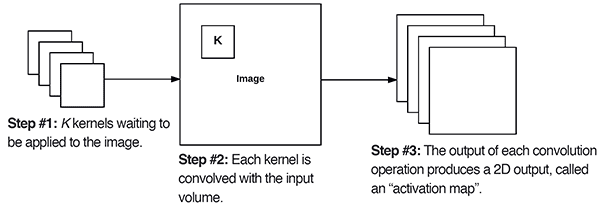
\includegraphics[width=0.6\textwidth]{rapport/plots/keras_conv2d_num_filters.png}
                \caption{Modèle de réseau convolutionnel en 2 dimensions}
            \end{figure}
            
            Cette couche, est la première de chaque bloc de notre réseau. Elle va récupérer depuis l'image toutes les caractéristiques en les faisant convoluer. Ici nous pouvons faire varier plusieurs paramètres importants\space:
            
            \begin{itemize}
                \item le paramètre \textit{kernel\_size} représente la taille de chaque kernel qui va convoluer. Les différentes valeurs de taille que nous avons testées sont les tuples impairs, de (1, 1) jusqu'à (7, 7). Au-dessus de (7, 7) les performances chutes. Les kernels étant trop gros, on perd la qualité de la convolution. Nous avons choisi des tuples impairs car c'étaient les valeurs recommandées par le tutoriel\cite{convdLayer} sur les Conv2D proposées dans le sujet. Il recommande aussi, pour des images supérieur ou égales à 120x120 de commencer par une taille de kernel supérieur ou égale à \textbf{(3, 3)}. Nous avons donc pris cette valeur comme base.
                
                \item le paramètre \textit{filters} représente le nombre de kernels qui vont passer sur l'image. Ici les valeurs de filters sont des puissances de 2, allant de 16 à 1024. Il est conventionnel d'augmenter d'une puissance de 2 le nombre de kernels, en allant en profondeur dans le réseau. Le tutoriel\cite{convdLayer} proposé par le sujet nous recommande de commencer par des valeurs comprises entre 32 et 128, et de finir par des valeurs entre 256 et 1024. Nous sommes donc restés sur cette échelle.

            \end{itemize}
        
            \subsubsection{\href{https://keras.io/api/layers/pooling_layers/max_pooling2d/}{MaxPooling2D}}
            Une fois la convolution effectuée, il est nécessaire de réduire la taille des entrées. Comme précisé dans le sujet, nous avons utilisé le maximum plutôt que la moyenne. En effet le \textit{maxpooling} va extraire les caractéristiques les plus importantes de l'image. Ici les valeurs sont de \textbf{(2, 2)} pour la \textit{\textbf{poolsize}}. En sachant que cette valeur réduit \textbf{75\%} des données, augmenter la valeur n'est pas réellement utile. Nous avons tout de même essayer de la faire varier pour en voir les conséquences. Mais nous avons vite vu que la perte d'informations devient trop importante.
            
            \subsubsection{\href{https://keras.io/api/layers/regularization_layers/dropout/}{Dropout}}
            Le layer \textit{\textit{dropout}} est utile afin d'éviter l'\textit{overfitting} de notre réseau. La valeur que l'on fait varier, \textit{rate}, représente la probabilité pour un lien entre deux neurones d'être temporairement désactivé. Ici l'intervalle de valeurs se situe entre 0 et 1. Cependant 0 et 1 n'étant pas réellement utiles, nous avons fait varier les valeurs de 0.1 à 0.9. Étant donné qu'à chaque époque, les neurones ayant été désactivés peuvent être réactivés, les chances d'\textit{overfitting} sont réduites.
        
            \subsubsection{\href{https://keras.io/api/layers/core_layers/dense/}{Dense}}
            Le layer \textit{Dense} est une couche de neurones qui va être connectée à tous les précédents neurones du réseau. Il est important, car il récupère toutes les valeurs des précédents neurones. Dans ce réseau, on peut préciser la valeur \textit{units} qui va donner la taille de la sortie du réseau. C'est important, car en fonction du nombre de classes à prédire, le dernier layer doit être un \textit{Dense} avec une valeur d'\textit{units} adapté au problème. Ici pour notre classificateur, nous laissons un \textit{Dense} avec units à \textbf{1}. Dans les exemples que nous trouvions sur internet, ils ajoutés la plupart du temps un ou deux layers \textit{dense} avec une units multiple de 2 entre 64 et 512. Nous allons donc tester des valeurs dans cette échelle. 
        
            \subsubsection{\href{https://keras.io/api/models/sequential/}{Flatten}}
            Nous avons rajouté la couche \textit{Flatten}, après avoir lu quelques articles précisant que cette couche permettait de redimensionner les tensors. En effet, nous ne pouvions pas compiler notre modèle dans celui ci, car les dimensions entre les dernières couches ne correspondait pas. Nous nous sommes grandement inspirés de modèles déjà construits, et nous avons pu observer que cette couche était placée juste avant les dernières couches de \textit{Dense}.
            
            \subsubsection{\href{https://keras.io/api/models/sequential/}{Sequential}}
            Enfin nous avons utilisé un modèle séquentiel, afin de pouvoir déclarer à la suite toutes nos couches. C'est un modèle qui est le plus communément utilisé dans la reconnaissance d'images.
            
            \subsubsection{Fonctions d'activation}
            
            Il y a plusieurs fonctions d'activation possible pour chacune des couches. Mais principalement, nous pouvons énumérer la fonction \textit{ReLU}, \textit{softmax} et \textit{sigmoid}. 
            
            La \textit{Rectified Linear Unit} (ReLU) est la fonction d'activation la plus communément utilisée. En effet elle permet à chaque neurones d'éviter toutes valeur négative.
            
            Enfin pour le tout dernier Layer de \textit{Dense}, nous avions le choix entre la fonction \textit{\textbf{sigmoid}} et \textit{\textbf{softmax}}. La fonction \textit{sigmoid} est utilisée quand le nombre de classes à prédire est binaire. Sinon nous utilisons la fonction \textit{softmax}. Nous avons opté pour la première en raison de notre problème.
        
    \section{Expérimentations}
        
        \subsection{Recherche d'une base}
        Nous allons ici rechercher une base proposant des résultats encourageants, sur laquelle faire nos différentes expérimentations. Voici les modèles étudiés :
        \begin{enumerate}
            \item \begin{itemize}
                \item \textbf{1 Conv2D} avec un \textbf{\textit{filters} égal à 64}.
                \item Un \textbf{MaxPooling2D de \textit{pool\_size} (2, 2)}.
                \item Un \textbf{dropouts de rate 0.3}.
                \item Une couche de \textit{\textbf{Flatten}}.
                \item \textbf{Deux layers \textit{Dense}}, dont un d'\textit{units} \textbf{32} avec une fonction d'activation \textit{"ReLU"}, et le dernier en \textbf{1} avec une fonction \textit{"sigmoid"}.
            \end{itemize}
            
            \item Nous avons ajouté un deuxième bloc (Conv2, MaxPooling, dropouts).
            
            \item Nous avons encore ajouté un troisième bloc.
            
            \item Nous avons ajouté un quatrième bloc.
            
            \item Nous avons ajouté un troisième dense, il sera connecté en premier à la sortie et a son units de taille 256 avec une fonction d'activation \textit{"ReLU"}.
            
            \item Nous modifions le dense précédemment ajouté, et changeons le 256 en 512.
        \end{enumerate}
        
        \begin{figure}[H]
            \centering
            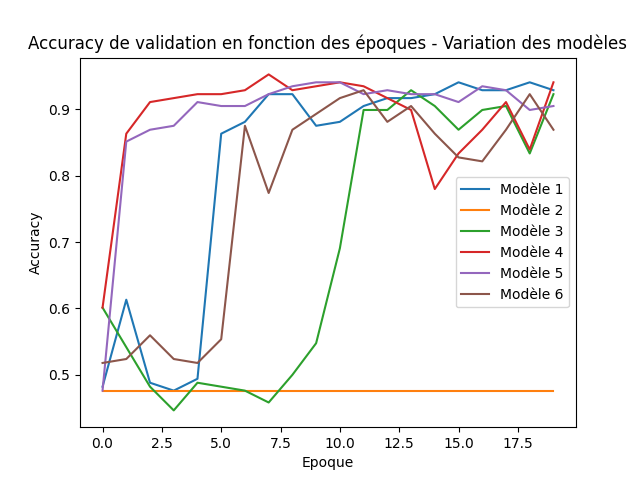
\includegraphics[width=0.7\textwidth]{rapport/plots/model_acc.png}
            \caption{Variation du val\_acc en fonction des modèles}
            \label{fig:mesh1_model}
        \end{figure}

        \begin{figure}[H]
            \centering
            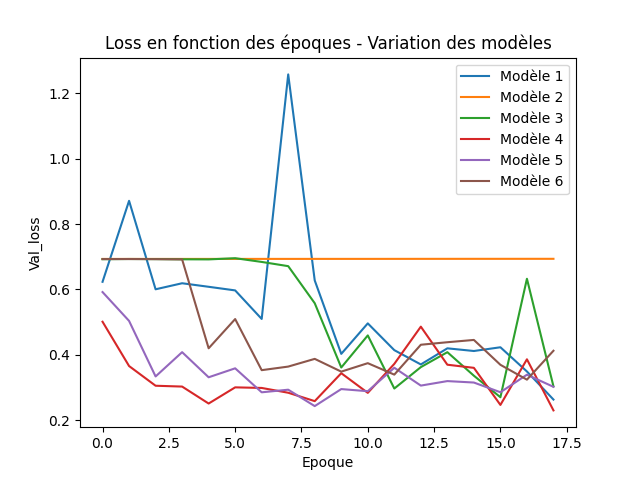
\includegraphics[width=0.7\textwidth]{rapport/plots/model_loss.png}
            \caption{Variation du val\_loss en fonction des modèles}
            \label{fig:mesh2_model}
        \end{figure}
        
        À partir de ces résultats, nous avons opté pour la cinquième courbe, qui possède de bonnes valeurs, ainsi qu'une évolution stable et cohérente.
        
        \newpage
        \subsection{Variation du kerner\_size}
        Le guide proposé par le sujet nous indiquait d'utiliser des valeurs tuples impairs, entre (1, 1) et (7, 7). Voici nos expérimentations :
        
        \begin{figure}[H]
            \centering
            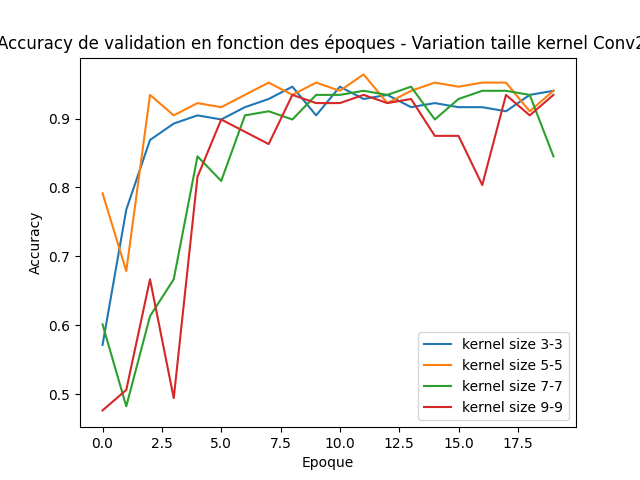
\includegraphics[width=0.65\textwidth]{rapport/plots/kernel_acc.png}
            \caption{Variation du val\_acc en fonction du kernel\_size}
            \label{fig:mesh1}
        \end{figure}

        \begin{figure}[H]
            \centering
            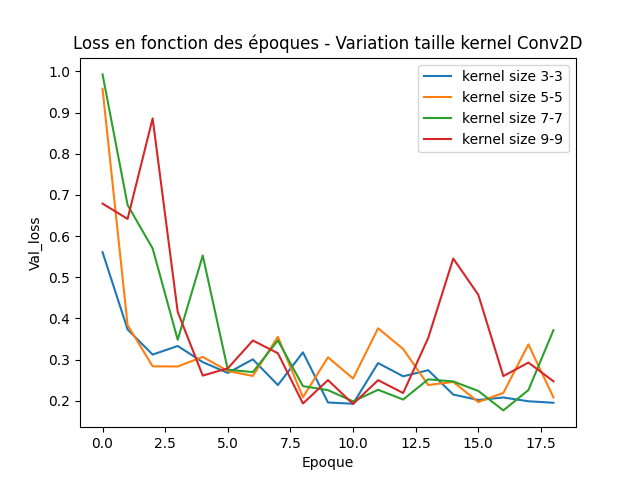
\includegraphics[width=0.65\textwidth]{rapport/plots/kernel_loss.png}
            \caption{Variation du val\_loss en fonction du kernel\_size}
            \label{fig:mesh2}
        \end{figure}
        
        Nous pouvons ainsi constater que le choix vers lequel nous pouvons nous porter est celui de la courbe bleue, c'est à dire un tuple (3, 3). Elle est la plus précise possible, faisant jeu égal avec quelques autres mais se démarque particulièrement au niveau des pertes, ou elle est la plus basse de toutes.
        
        \newpage
        \subsection{Variation des filters}
        Les guides nous recommandait de commencer par des valeurs entre 32 et et 128, et de terminer par des valeurs entre 256 et 1024. Voici nos résultats.
        
        \begin{figure}[H]
            \centering
            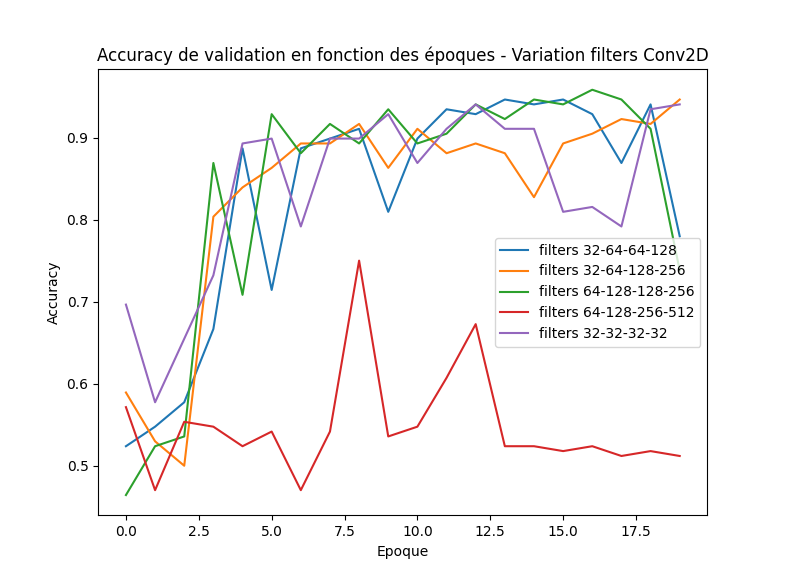
\includegraphics[width=0.65\textwidth]{rapport/plots/filters_acc.png}
            \caption{Variation du val\_acc en fonction de la taille des filters}
            \label{fig:mesh1}
        \end{figure}

        \begin{figure}[H]
            \centering
            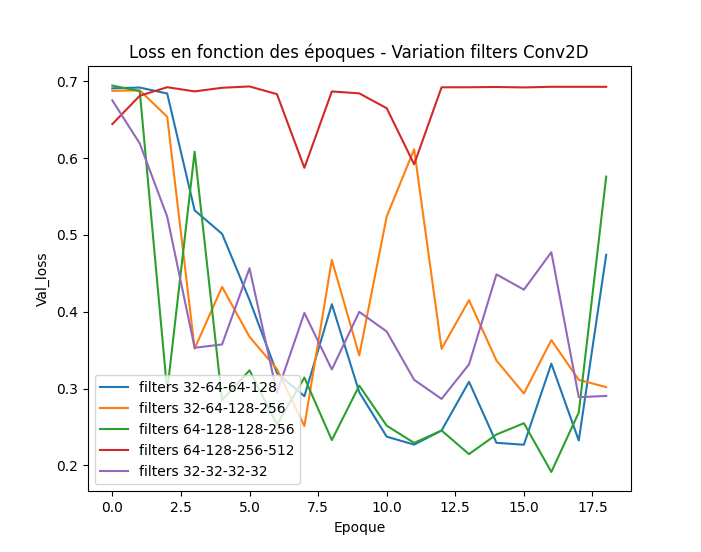
\includegraphics[width=0.65\textwidth]{rapport/plots/filters_loss.png}
            \caption{Variation du val\_loss en fonction de la taille des filters}
            \label{fig:mesh2}
        \end{figure}
        
        Nous pouvons déduire que le meilleur rapport est celui de la courbe orange : 32, 64, 128, 256. Nous pouvons également remarquer que la courbe rouge présente des résultats catastrophique : les valeurs commencent et finissent peut-être trop haut.
        
        \subsection{Variation des dropouts}
        Nous avions expliqué que nous allions utiliser des valeurs entre 0.1 et 0.9 : voici nos expérimentations.
        
        \begin{figure}[H]
            \centering
            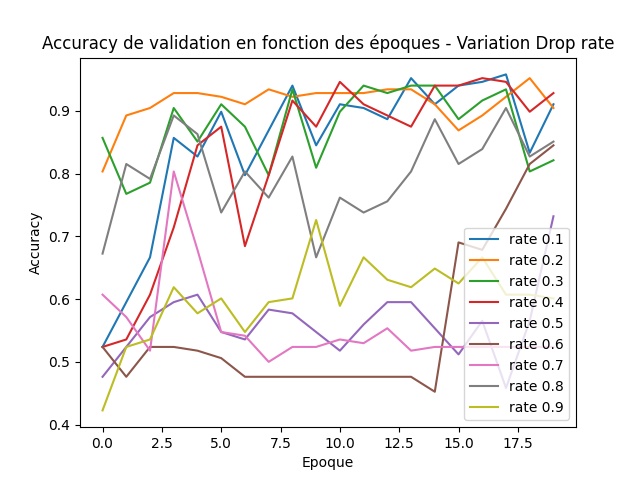
\includegraphics[width=0.7\textwidth]{rapport/plots/dropoutr_acc.png}
            \caption{Variation du val\_acc en fonction du dropouts rate}
            \label{fig:mesh1}
        \end{figure}

        \begin{figure}[H]
            \centering
            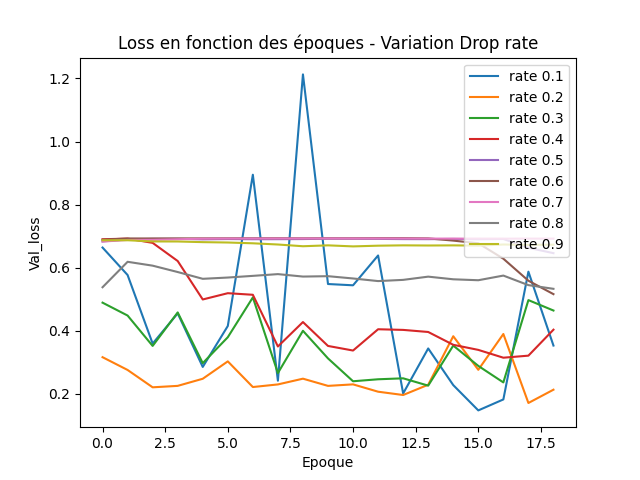
\includegraphics[width=0.7\textwidth]{rapport/plots/dropout_loss.png}
            \caption{Variation du val\_loss en fonction du dropouts rate}
            \label{fig:mesh2}
        \end{figure}
        
        Grâce à ces résultats, nous déduisons que la courbe \textbf{orange}, qui est dans le top des plus précises tout en ayant les plus basses pertes, est la meilleure. Le meilleur \textit{rate} est donc \textbf{0.2}.
        
        \subsection{Variation des Dense Units}
        Au niveau des layers Dense et de leurs units, nous avons comme expliqué précédemment fais varier les taille de ces derniers entre \textbf{64} et \textbf{512}. Nous avons aussi tenté plusieurs nombres de layers, entre \textbf{1} et \textbf{3}.
        
        \begin{figure}[H]
            \centering
            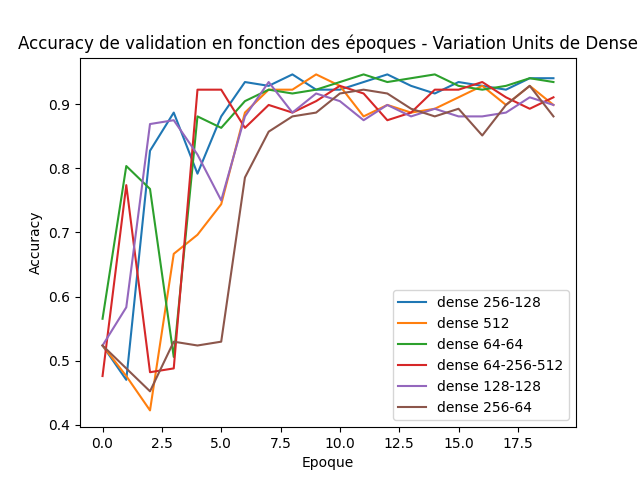
\includegraphics[width=0.7\textwidth]{rapport/plots/dense_acc.png}
            \caption{Variation du val\_acc en fonction du nombre de layers Dense et de leurs tailles}
            \label{fig:mesh1}
        \end{figure}

        \begin{figure}[H]
            \centering
            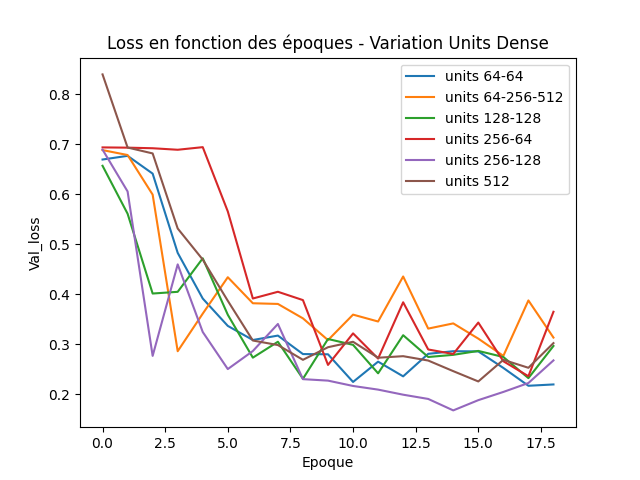
\includegraphics[width=0.7\textwidth]{rapport/plots/dense_loss.png}
            \caption{Variation du val\_loss en fonction du nombre de layers Dense et de leurs tailles}
            \label{fig:mesh2}
        \end{figure}
        
        Nous pouvons déduire à partir de ces données que le meilleur choix est celui de la courbe \textbf{bleue}, deux layers de tailles respectives \textbf{256} et \textbf{128}.
    
        \subsection{Résultats obtenus}
        Une fois toutes ces expérimentations effectuées, nous avons pu trouver notre modèle optimal. Au final voici les performances de notre modèle sur un jeu de données d'environ 600 images\space:
        
        Nous avons retenu le modèle 5 \ref{fig:mesh1_model} avec les paramètres suivants:
        
        \begin{itemize}
            \item \textit{Conv2D} avec 4 filters différents, dans l'ordre \textbf{32}, \textbf{64}, \textbf{128} puis Quatre \textbf{256}. Un kernel\_size de \textbf{(3, 3)}. Une fonction d'activation "ReLU".
            
            \item Trois \textit{MaxPooling} avec un \textit{pool\_size} de \textbf{2x2}.
            
            \item Quatre layers\textit{Dropout} avec une valeur \textit{rate} de \textbf{0.2}.
            
            \item Deux layers \textit{Dense} avec respectivement \textbf{256}, \textbf{128} en units et une fonction d'activation \textbf{"ReLU"}. Ainsi qu'un dernier layer Dense d'units \textbf{1} avec une fonction d'activation \textbf{"sigmoid"}.
        \end{itemize}
        
        \begin{figure}[H]
            \centering
            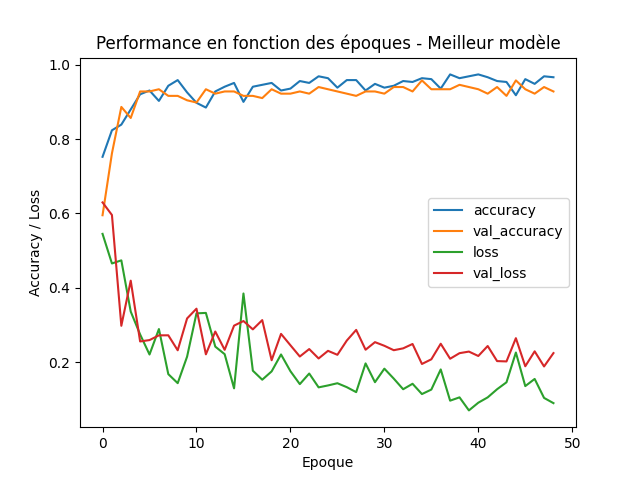
\includegraphics[width=0.7\textwidth]{rapport/plots/best.png}
            \caption{Performances du modèles retenus.}
            \label{fig:mesh1}
        \end{figure}
     
     \clearpage   
    Au final, lorsque l'on teste de nouvelles images, notre modèle reconnaît assez bien les personnes avec masque et sans masque. Les cadres proposés sont ainsi la plus part du temps vrais. Cependant nous avons un problème dans un cas similaire à cette prédiction \ref{fig:profile} :
    
    \begin{figure}[h]
        \centering
        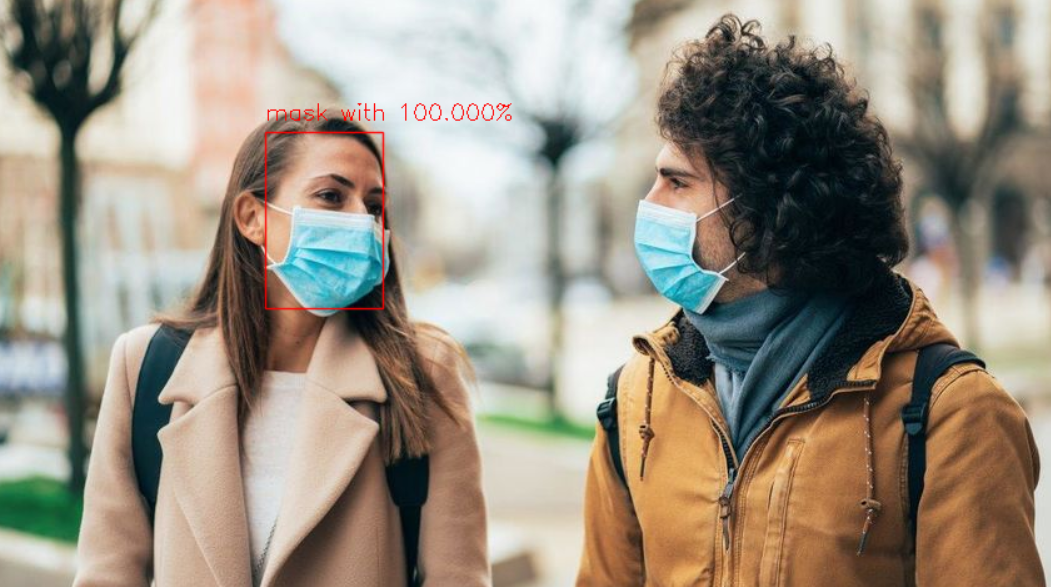
\includegraphics[width=0.6\textwidth]{rapport/img/demiface.png}
        \caption{Prédiction d'une image avec une personne de profile}
        \label{fig:profile}
    \end{figure}
    
    On remarque que la personne de profil n'est pas considérée comme une personne portant un masque. En effet ce problème provient du manque de donnée similaire lors de notre entraînement. Le problème est le même avec des personnes sans masque.
    
    \section{Problèmes rencontrés}
    Nous avons rencontrés durant cette seconde partie divers problèmes ayant perturbé notre entraînement et la précision finale de notre programme. Nous allons ici les énumérer.

        \subsection{Portabilité}
        Dans la continuité de la partie 1, nous n'arrivons pas a lancer le programme sur Mac M1. Une \textbf{"illegal hardware exception"} apparaît. Nous nous en sommes rendu compte le jour du rendu. Il faut que nous étudions sur Tensorflow est compatible avec l'architecture ARM ou non. Il y a peut-être des moyens de régler ce souci mais nous n'avons pas eu vraiment le temps de traiter ce problème.
        
        \subsection{Overfitting}
        Nous avons été confrontés au début à un sérieux problème d'\textit{overfitting}. En effet, nous étions beaucoup trop laxistes sur le cadrage de nos annotations, laissant place ainsi à beaucoup trop de bruit dans chaque image. Cela nous a donné par conséquent des résultats assez hasardeux dans nos prédictions. C'est pourquoi nous avons par la suite décidé de bien s'appliquer sur tous nos cadres et de n'encadrer que le strict nécessaire, le visage. Nous évitons les cheveux, les chapeaux, et les arrière-plan du mieux que nous le pouvons. Après avoir re-traité toutes nos données, nous avons obtenu de meilleurs résultats.
        
        \subsection{Underfitting}
        De la même manière, nous avons également rencontré au début un problème d'\textit{underfitting}. En effet, pendant un moment, notre dataset était constitué uniquement de visage de face et de la même ethnie. Ce qui a causé problème : notre fonction de prédiction penait à détecter les visages de côté, d'autres ethnies, avec lunettes et autres. C'est pourquoi nous avons pris le soin d'assembler plusieurs types de visages, des deux sexes, avec et sans accessoires.
        
        \subsection{Pertinence du dataset}
        Nous avons quelques soucis avec nos données par exemple au niveau des masques de couleurs. Notre fonction de prédiction a souvent des difficultés à reconnaître les masques de couleur verte, jaunes et autres masques atypiques. Nous ne l'avons entraîné que sur des masques standard (bleus, blancs, noirs). Nous étions assez gênés sur ce point et avons eu du mal à rendre nos fonctions plus flexibles tout en gardant sa stabilité. 

        La fonction nécessite également qu'on lui envoie des échantillons bien cadrés, ce que fait heureusement parfaitement notre fonction de détection. Mais avec par exemple les cadrages hasardeux de notre précédente fonction de détection, avec la \textit{selective search d'Open CV}, elle avait beaucoup plus de mal.
        
        \subsection{Interprétation des résultats}
        Nous avions beaucoup eu de mauvaises interprétations de nos résultats. Parfois nous avions de l'\textit{overfitting} sans nous en rendre compte, également pour l'\textit{underfitting}, et parfois nous rentrions de mauvais paramètres dans notre modèle. Car nous maîtrisions mal notre sujet au début, mais heureusement, ce n'était que le but de ce projet. Nous avons au fur et à mesure progressé et appris à détecter les incohérences d'un modèle dans ses résultats. Par exemple, nous avons compris que si lors de l'entraînement, au fur et à mesure des époques, notre \textit{\textbf{loss}} continuait de décroître mais que le \textit{\textbf{val\_loss}} continuait de rester stable voire accroître, alors cela était généralement signe d'\textit{overfitting}.
        
        
    \clearpage
\part{Conclusion}
    
    \section{Possibilités d'améliorations du logiciel}
    Notre logiciel a encore une énorme marge de progression. Nous avons, comme évoqué dans la première partie, plusieurs possibilités d'amélioration du confort d'utilisation et de l'ergonomie du logiciel. Nous pouvons implémenter plus de raccourcis claviers. Nous pouvons aussi ajouter de l'auto-complétion des annotations (la plus récente). Il y a aussi le souci de la barre de progression sur \textbf{mac OS} que nous devons régler. Le chargement d'un projet bien fourni en images peut aussi prendre quelques secondes : nous pourrions ajouter une barre de progression pour faire patienter l'utilisateur. Il serait aussi intéressant d'étudier si nous pouvons implémenter un mécanisme de sauvegarde automatique ne plombant pas nos performances.
    Un petit regret que nous avons est notre manque d'utilisation de tests unitaires : nous avons découvert leur utilité ce semestre, mais avons eu l'arrogance de nous en passer sur ce projet. Les utiliser aurait peut-être pu réduire et anticiper pas mal de bug que nous avons eu au cours du développement.
    
    Nous pouvons aussi améliorer l'intégration du classificateur au logiciel. Elle fonctionne, mais peut encore être rendue bien plus naturelle. Nous avons eu quelques problèmes dessus, la faute à notre manque d'expérience dans le \textit{\textbf{multithreading}} en \textit{Python}.
    
    \section{Possibilités d'améliorations du Classificateur}
    Nous pouvons encore améliorer notre fonction de prédiction. Lui faire reconnaître de manière beaucoup plus stable les masques atypiques, ainsi que les visages qui sont en très basse résolution, dont elle a parfois du mal à détecter. Nous pouvons aussi faire en sorte que le script de pré-traitement des données n'ait pas à importer \textit{Tensorflow} au démarrage, le rendant plus rapide à lancer. 
    Ensuite, nous pouvons évidemment pousser nos tests encore plus loin, et tester encore plus de valeurs, améliorant ainsi toujours plus notre fonction de prédiction.
    Nous pouvons aussi continuer de creuser pour voir s'il est possible de détecter les visages sans utiliser de modèle pré-entraîné.
    Enfin, nous pouvons régler les soucis de portabilité sur les Mac M1.
    
    \section{Mots de la fin}
    Nous avons beaucoup apprécié travaillé sur ce projet. Un sentiment de satisfaction s'en dégage, nous avons créé un logiciel de toute pièce, appris à utiliser des librairies très utiles, que ce soit pour les interface graphiques ou la manipulation d'image, et avons manipulé de manière concrète le domaine du machine learning. C'est un projet dont nous sommes fier et qui nous a beaucoup appris. Nous avons grâce à cette matière dorénavant plusieurs idées de projet d'entraînement d'intelligence artificielle que nous avons hâte de tester.
    
\newpage
\printbibliography{}
    

\end{document}
